% Szglab4
% ===========================================================================
%
\chapter{Szkeleton tervezése}

\thispagestyle{fancy}

\section{A szkeleton modell valóságos use-case-ei}
%\comment{A szkeletonnak, mint önálló programnak a működésével kapcsolatos use-case-ek.}

\subsection{Use-case diagram}

\begin{figure}[H]
\begin{center}
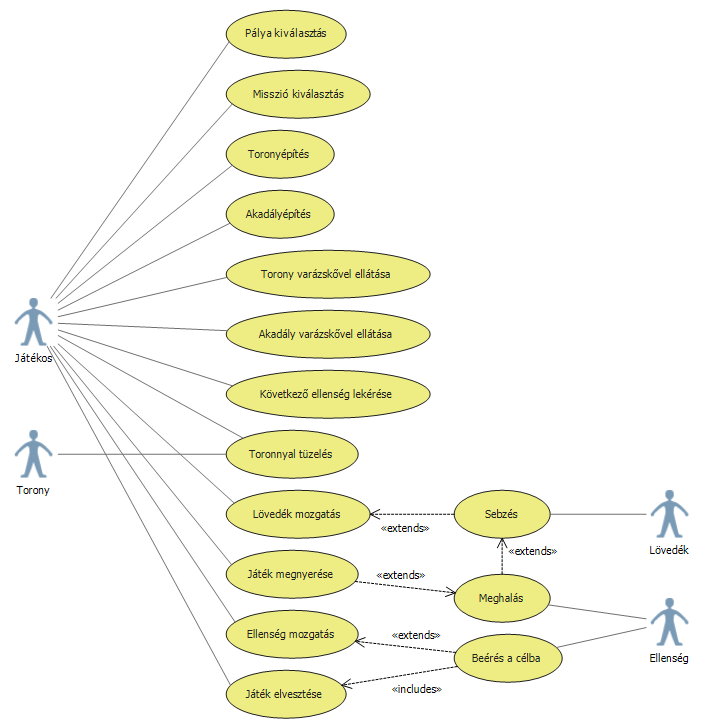
\includegraphics[width=17cm]{images/skeleton_use_case.png}
\caption{Use case diagram}
\label{fig:SzkeletonUseCase}
\end{center}
\end{figure}

\pagebreak

\subsection{Use-case leírások}
%\comment{Minden use-case-hez külön}

%Use-case neve  Rövid leírás  Aktorok  Forgatókönyv 

\usecase{Pálya kiválasztás}
{A felhasználó kiválaszt egy pályát.}
{Felhasználó}
{A program felkínál egy listát az elérhető pályák neveiről, amelyből a felhasználó kiválasztja azt, amelyiken játszani szeretne.}

\usecase{Misszió kiválasztás}
{A felhasználó kiválaszt egy missziót.}
{Felhasználó}
{A program felkínál egy listát az előzőleg kiválasztott pályán elérhető missziók neveiről, amelyből a felhasználó kiválasztja azt, amelyiken játszani szeretne.}

\usecase{Toronyépítés}
{A felhasználó felépít egy tornyot.}
{Felhasználó}
{A felhasználó megad egy pozíciót, ahova felépül egy torony.}

\usecase{Akadályépítés}
{A felhasználó felépít egy akadályt.}
{Felhasználó}
{A felhasználó megad egy pozíciót, ahova felépül egy akadály.}

\usecase{Torony varázskővel ellátása}
{A felhasználó ellát egy tornyot egy varászkővel.}
{Felhasználó}
{A felhasználó kiválaszt egy tornyot, majd egy varázskövet, amivel a toronyot erősíti.}

\usecase{Akadály varázskővel ellátása}
{A felhasználó ellát egy akadályt egy varázskővel.}
{Felhasználó}
{A felhasználó kiválaszt egy akadályt, majd egy varázskövet, amivel az akadályt erősíti.}

\usecase{Következő ellenség lekérése}
{A misszió következő ellensége elindul.}
{Felhasználó}
{A misszió soron következő ellensége létrejön, és elindul a pályán a célja felé.}

\usecase{Toronnyal tüzelés}
{Egy torony lő egyet.}
{Felhasználó, Torony}
{Egy kiválasztott torony kibocsát egy lövedéket egy megadott ellenség felé.}

\usecase{Ellenség mozgatás}
{Egy ellenség halad.}
{Ellenség}
{A kiválasztott ellenség megtesz egy lépést a célja felé vezető úton.}

\usecase{Beérés a célba}
{Egy ellenség elérte a célt.}
{Ellenség}
{Egy ellenség mozgása után elérte a célt, így a játéknak vége.}

\usecase{Játék elvesztése}
{A játék véget ér.}
{Játékos}
{A játék befejeződik, a játékos vesztett}

\usecase{Lövedék mozgatás}
{Egy lövedék halad.}
{Lövedék}
{A kiválasztott lövedék megtesz egy lépést a célpontja felé.}

\usecase{Sebzés}
{Egy lövedék célt ér.}
{Lövedék}
{Egy lövedék mozgása közben elérte a célpontját, azt megsebezte.}

\usecase{Meghalás}
{Egy ellenség életereje elfogy.}
{Ellenség}
{Ha egy lövedék célba érésekor az ellenségnek kevesebb életereje van, mint amennyit a lövedék sebez, az ellenség meghal, eltűnik.}

\usecase{Játék megnyerése}
{Az utolsó ellenség is meghal.}
{Játékos}
{Egy ellenség halálakor a játékos megnyeri a játékot, ha nincs több ellenség életben.}

\section{A szkeleton kezelői felületének terve, dialógusok}
\comment{A szkeleton által elfogadott bemenetek , valamint a szöveges konzolon megjelenő kimenetek. A kiemenet formátuma olyan kell legyen, ami alapján a működés összevethető a korábbi szekvencia-diagramokkal.}

\section{Szekvencia diagramok a belső működésre}
\comment{A szkeletonban implementált szekvenciadiagramok. Tipikusan egy use-case egy diagram. Ezek megegyezhetnek a korábban specifikált diagramokkal, de az egyes életvonalakat (lifeline) egyértelműen a szkeletonban példányosított objektumokhoz kell tudni kötni. Azt kell megjeleníteni, hogy a szkeletonban létrehozott objektumok egymással hogyan fognak kommunikálni.}

\section{Kommunikációs diagramok}
\comment{A szkeletonban, az egyes szkeleton-use-case-ek futása során létrehozott objektumok és kapcsolataik bemutatására szolgáló diagramok. Ezek alapján valósítják meg a szkeleton fejlesztői az inicializáló kódrészleteket.}
